% TODO: Remove this and put it in the first page non summary
\setcounter{page}{1}
\section{Contexte}

\subsection{Activ'ESAIP}

Au cours de notre $4^{e}$ année de formation à l'\textsc{esaip}, nous sommes amenés à travailler en équipe d'étudiants, issus de différentes majeures, voire de différentes filières, dans le but de mener un projet ingénieur au sein d'une entreprise. Ce projet d'une durée de 5 semaines a pour objectif de nous professionnaliser tout en répondant à une problématique posée par l'entreprise.


\begin{figure}[!h]
    \centering
    
\includegraphics[scale=0.3]{img/activesaip.jpeg}
\end{figure}

\subsection{Panorama Performance}

Panorama Performance est une entreprise fondée en 2019 par Matthieu \textsc{Lecointre}, diplômé de l'école d'ingénieur angevine en sécurité environnement et prévention des risques ESAIP.\\
L'équipe de Panorama Performance s'est agrandie depuis sa création, car Alicia \textsc{Nodet}, chargée de la relation client, Julie \textsc{Oudard}, guide en haute performance et Nadine \textsc{Labbé} ont toutes trois rejoints l'entreprise.\\

Spécialisée dans l'amélioration performances des TPE et PME, Panorama Performance diagnostique, forme et accompagne les entreprises pour les faire progresser.\\

\begin{figure}[!h]
    \centering
    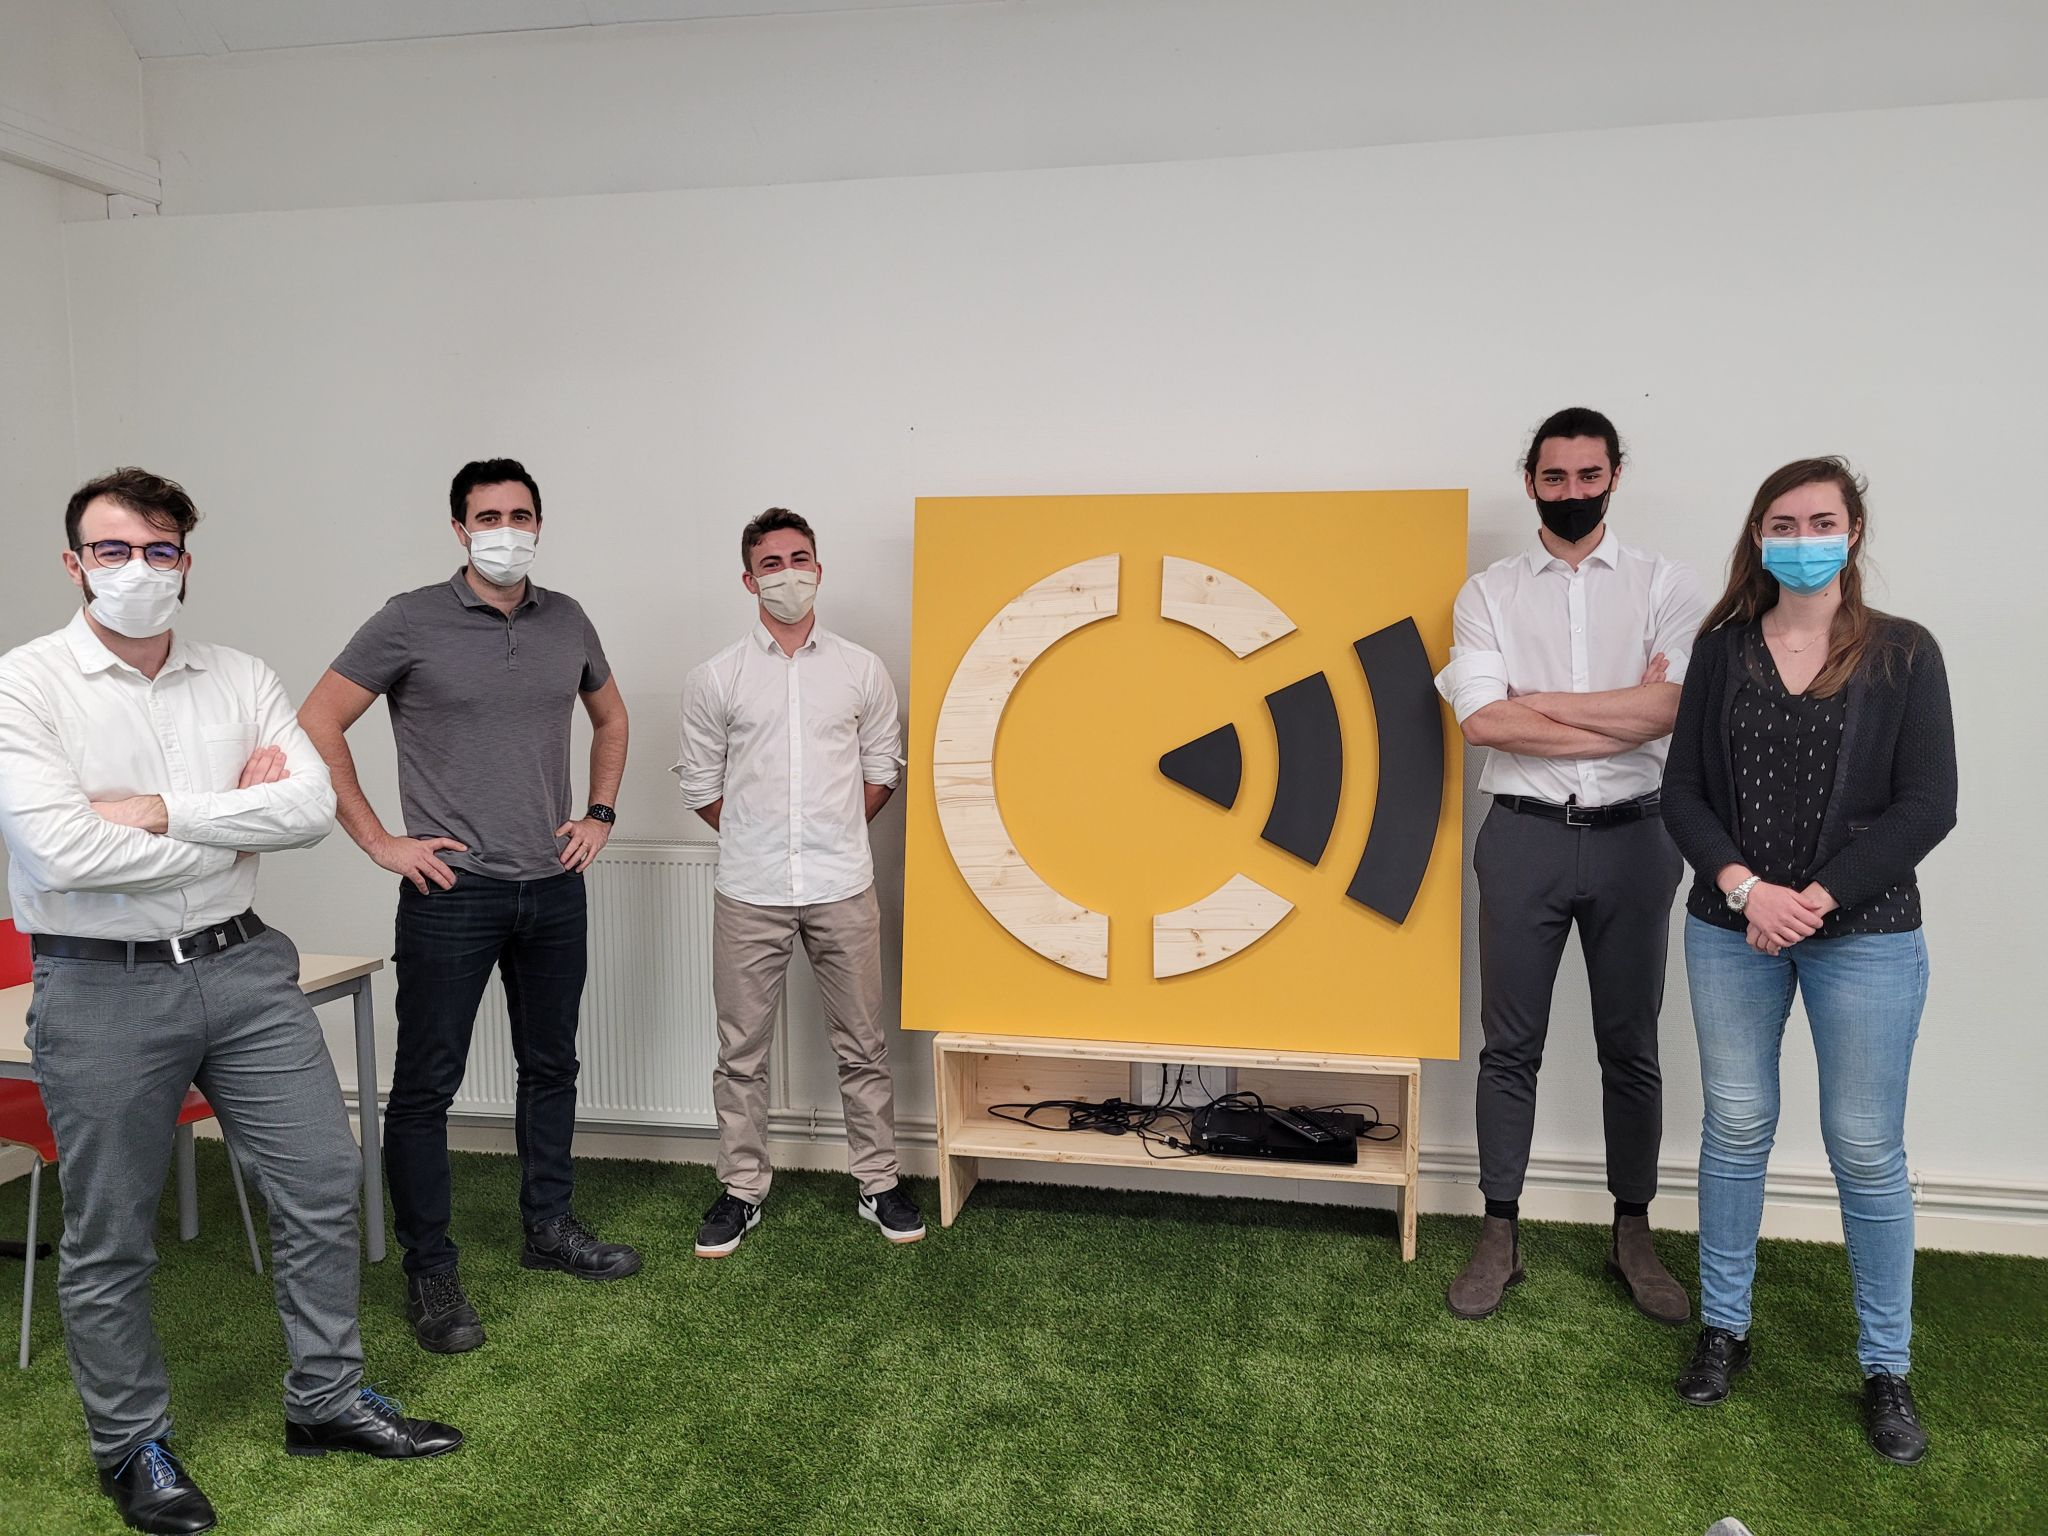
\includegraphics[scale=0.15]{img/team.jpg}
    \caption{\centering Équipe Activ'ESAIP, de gauche à droite: R. \textsc{Girou}, M. \textsc{Lecointre}, C. \textsc{Barbault}, V. \textsc{Carrillo}, J. \textsc{Oudard}}
    \label{fig:Equipe Activ'ESAIP}
\end{figure}

Pour aider les entreprises à s'améliorer, Panorama performance propose plusieurs accompagnements tels que le \textbf{diagnostic DRSO}, des formations en \textbf{Process Communication}, des \textbf{diagnostics de performance} ou encore des \textbf{accompagnements opérationnels}.\\

\clearpage
\subsection{La performance par le séquençage}

Un des outils que Panorama Performance propose aux entreprises suite à ses audits est le \textbf{séquenceur}. Cet outil a pour objectif de donner une vision globale de la charge de travail sur les deux semaines ou le mois qui vient. Panorama Performance adapte sa solution au cas par cas pour s'adapter aux besoins de chacune des entreprises qui s'en voit dotée ; c'est d'ailleurs un des points fort de l'accompagnement de Panorama Performance : la personnalisation de la solution.

\begin{figure}[!h]
    \centering
    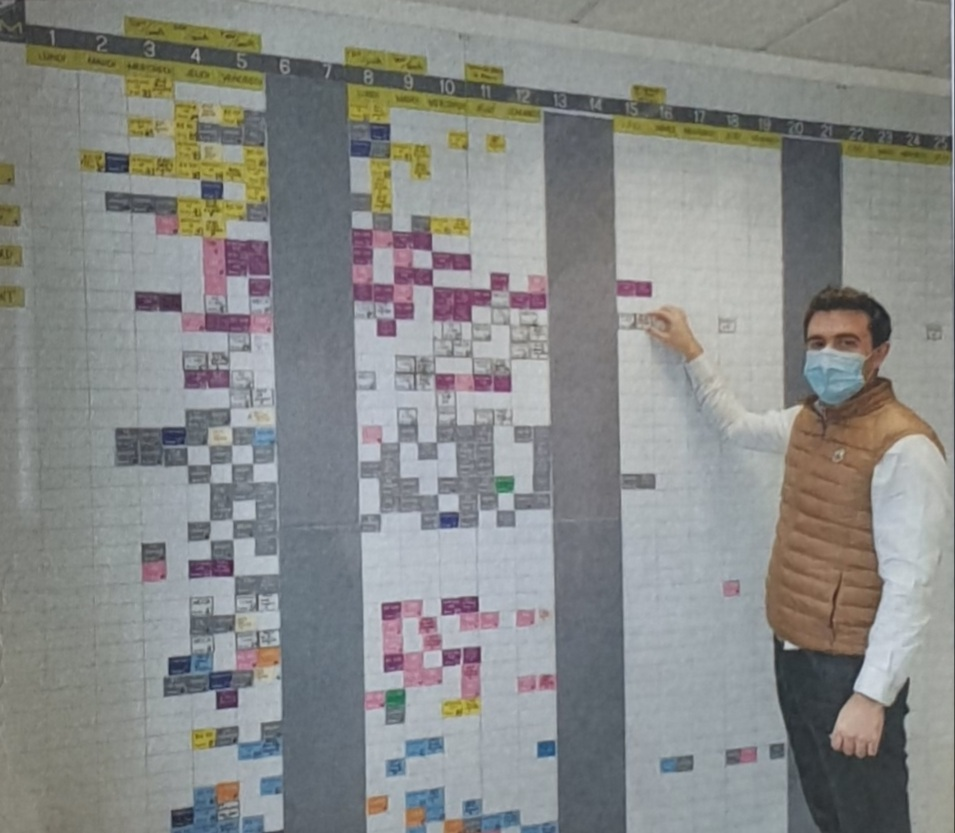
\includegraphics[scale=0.4]{img/sequenceur_2.jpeg}
    \caption{Le séquenceur, un outil d'aide à la performance industrielle}
    \label{fig:Séquenceur}
\end{figure}

De plus, cet outil de gestion de la planification industrielle est interactif : il permet à toute l'équipe de se retrouver afin de pouvoir interagir, communiquer et se mettre d'accord sur les modifications de planning à mettre en place\footnote{Lorsque l'équipe est adaptée à l'outil, seul le manager modifie le séquenceur et l'équipe n'a qu'à le consulter}.\\

\subsubsection*{Principe de fonctionnement}

Après une phase de prototypage de quelques jours, Panorama Performance cible les besoins de ses clients et construit ensuite avec eux un séquenceur. Sur ce séquenceur, on retrouve les commandes client (dans la figure \ref{fig:ProductionItem} elles sont placées dans une colonne à gauche) avec la référence de la pièce.\\

Le responsable vient ensuite placer dans la ligne correspondante toutes les étapes de fabrication nécessaires pour la commande (fraisage, tournage,\dots~cf. figure \ref{fig:productionLigne}). Ces étapes sont initialement les unes à la suite des autres, mais il les déplacera à une date antérieure si la charge de travail de la journée est trop importante ; de cette manière, la production est faite “Juste à temps" !\\

\begin{figure}[!h]
    \centering 
    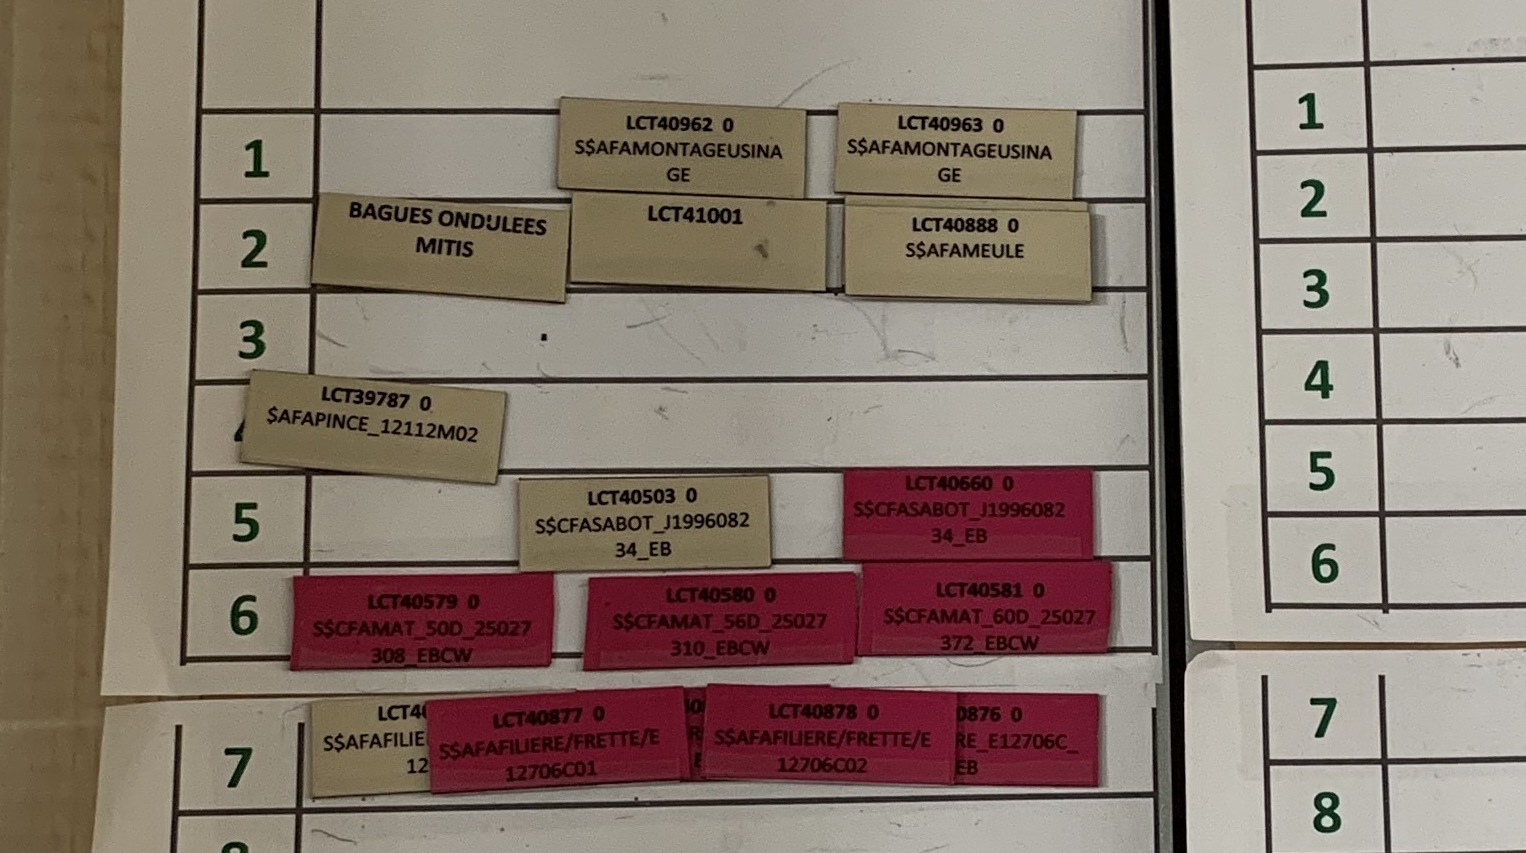
\includegraphics[scale=0.3]{img/productionItem.jpg}
    \caption{Les commandes sont ici placées à gauche}
    \label{fig:ProductionItem}
\end{figure}
\begin{figure}[!h]
    \centering
    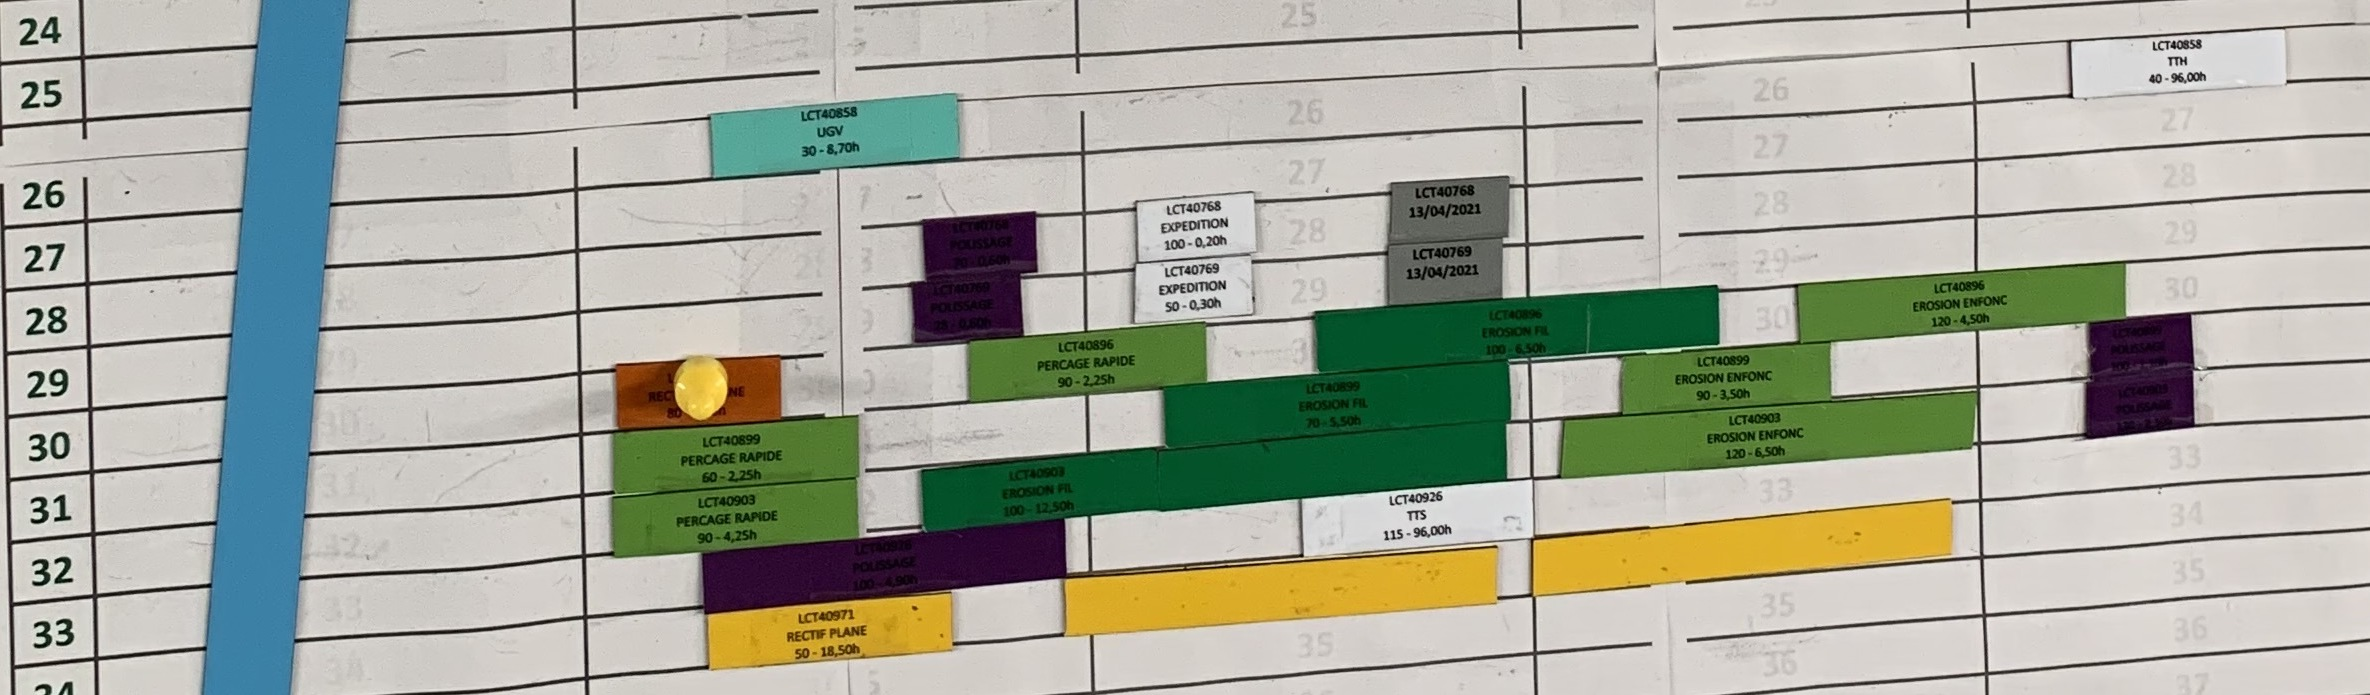
\includegraphics[scale=0.19]{img/ligne_production.jpg}
    \caption{Les lignes de production sont remplies avec les étapes de production}
    \label{fig:productionLigne}
\end{figure}   

Les cartes d'étapes de production ont une couleur associée à leur tâche, et une longueur variable en fonction de la charge horaire associée. Le nom de la compétence, la quantité de pièces à effectuer, la durée,\dots toutes ces informations figurent sur la carte, elles sont donc longues à réaliser à la main, et certains clients se dotent même d'imprimante à étiquette pour accélérer cette étape.
\hfill \\


\begin{figure}[!h]
    \centering
    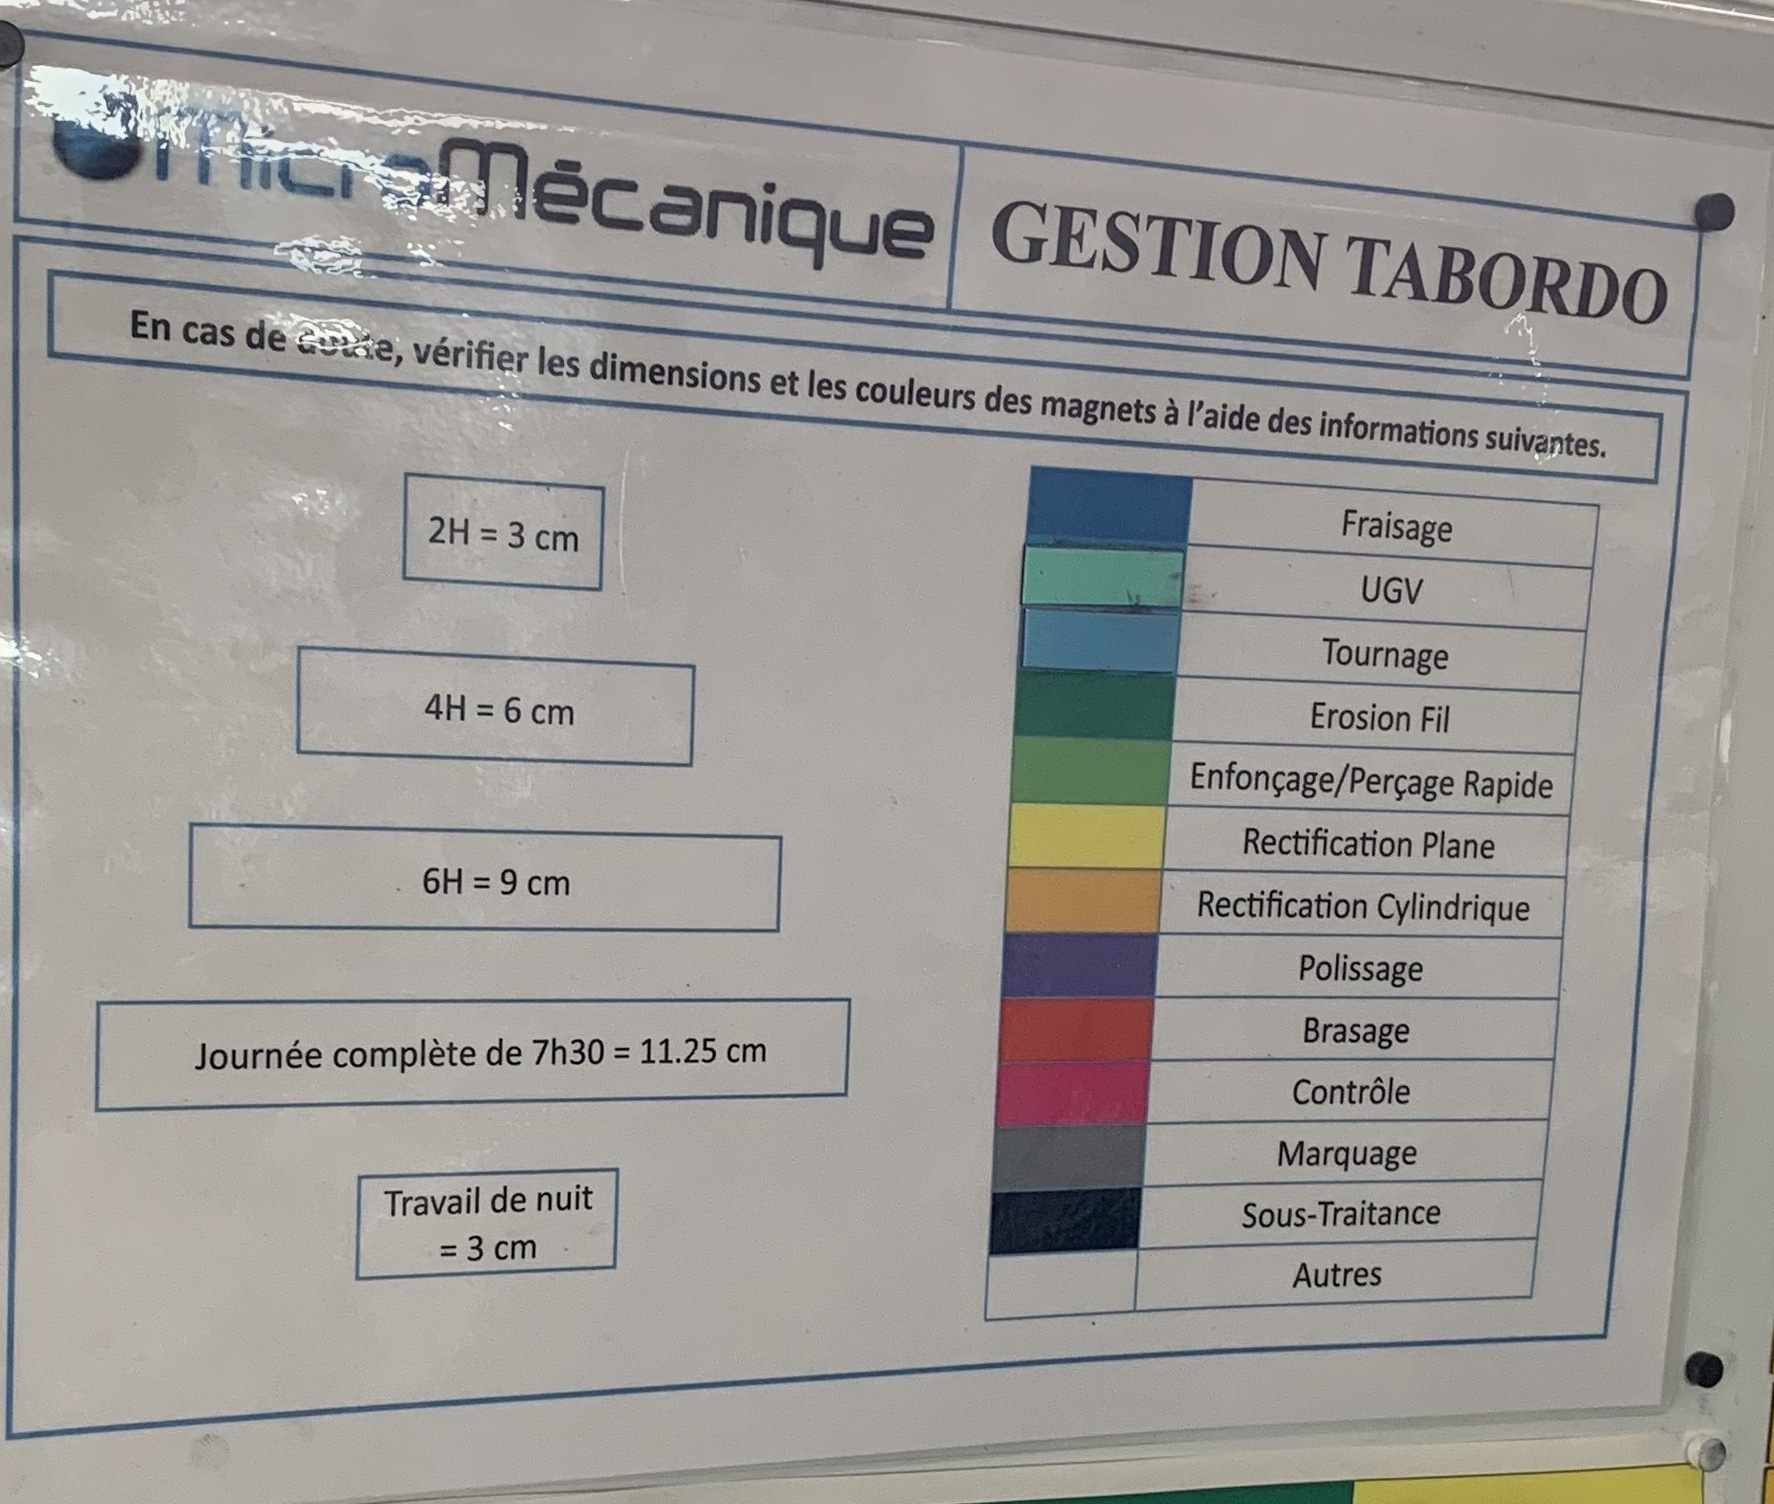
\includegraphics[scale=0.2]{img/productionStep.jpg}
    \caption{Les cartes d'étape de production suivent un design codifié (couleur, taille, contenu,\dots)}
    \label{fig:productionStep}
\end{figure}

Enfin, le manager peut placer des vignette (ici des épingles de couleur, cf. figures \ref{fig:productionLigne} et \ref{fig:employee}) pour signaler à chaque employé quelle sera sa mission du jour.

\begin{figure}[!h]
    \centering
    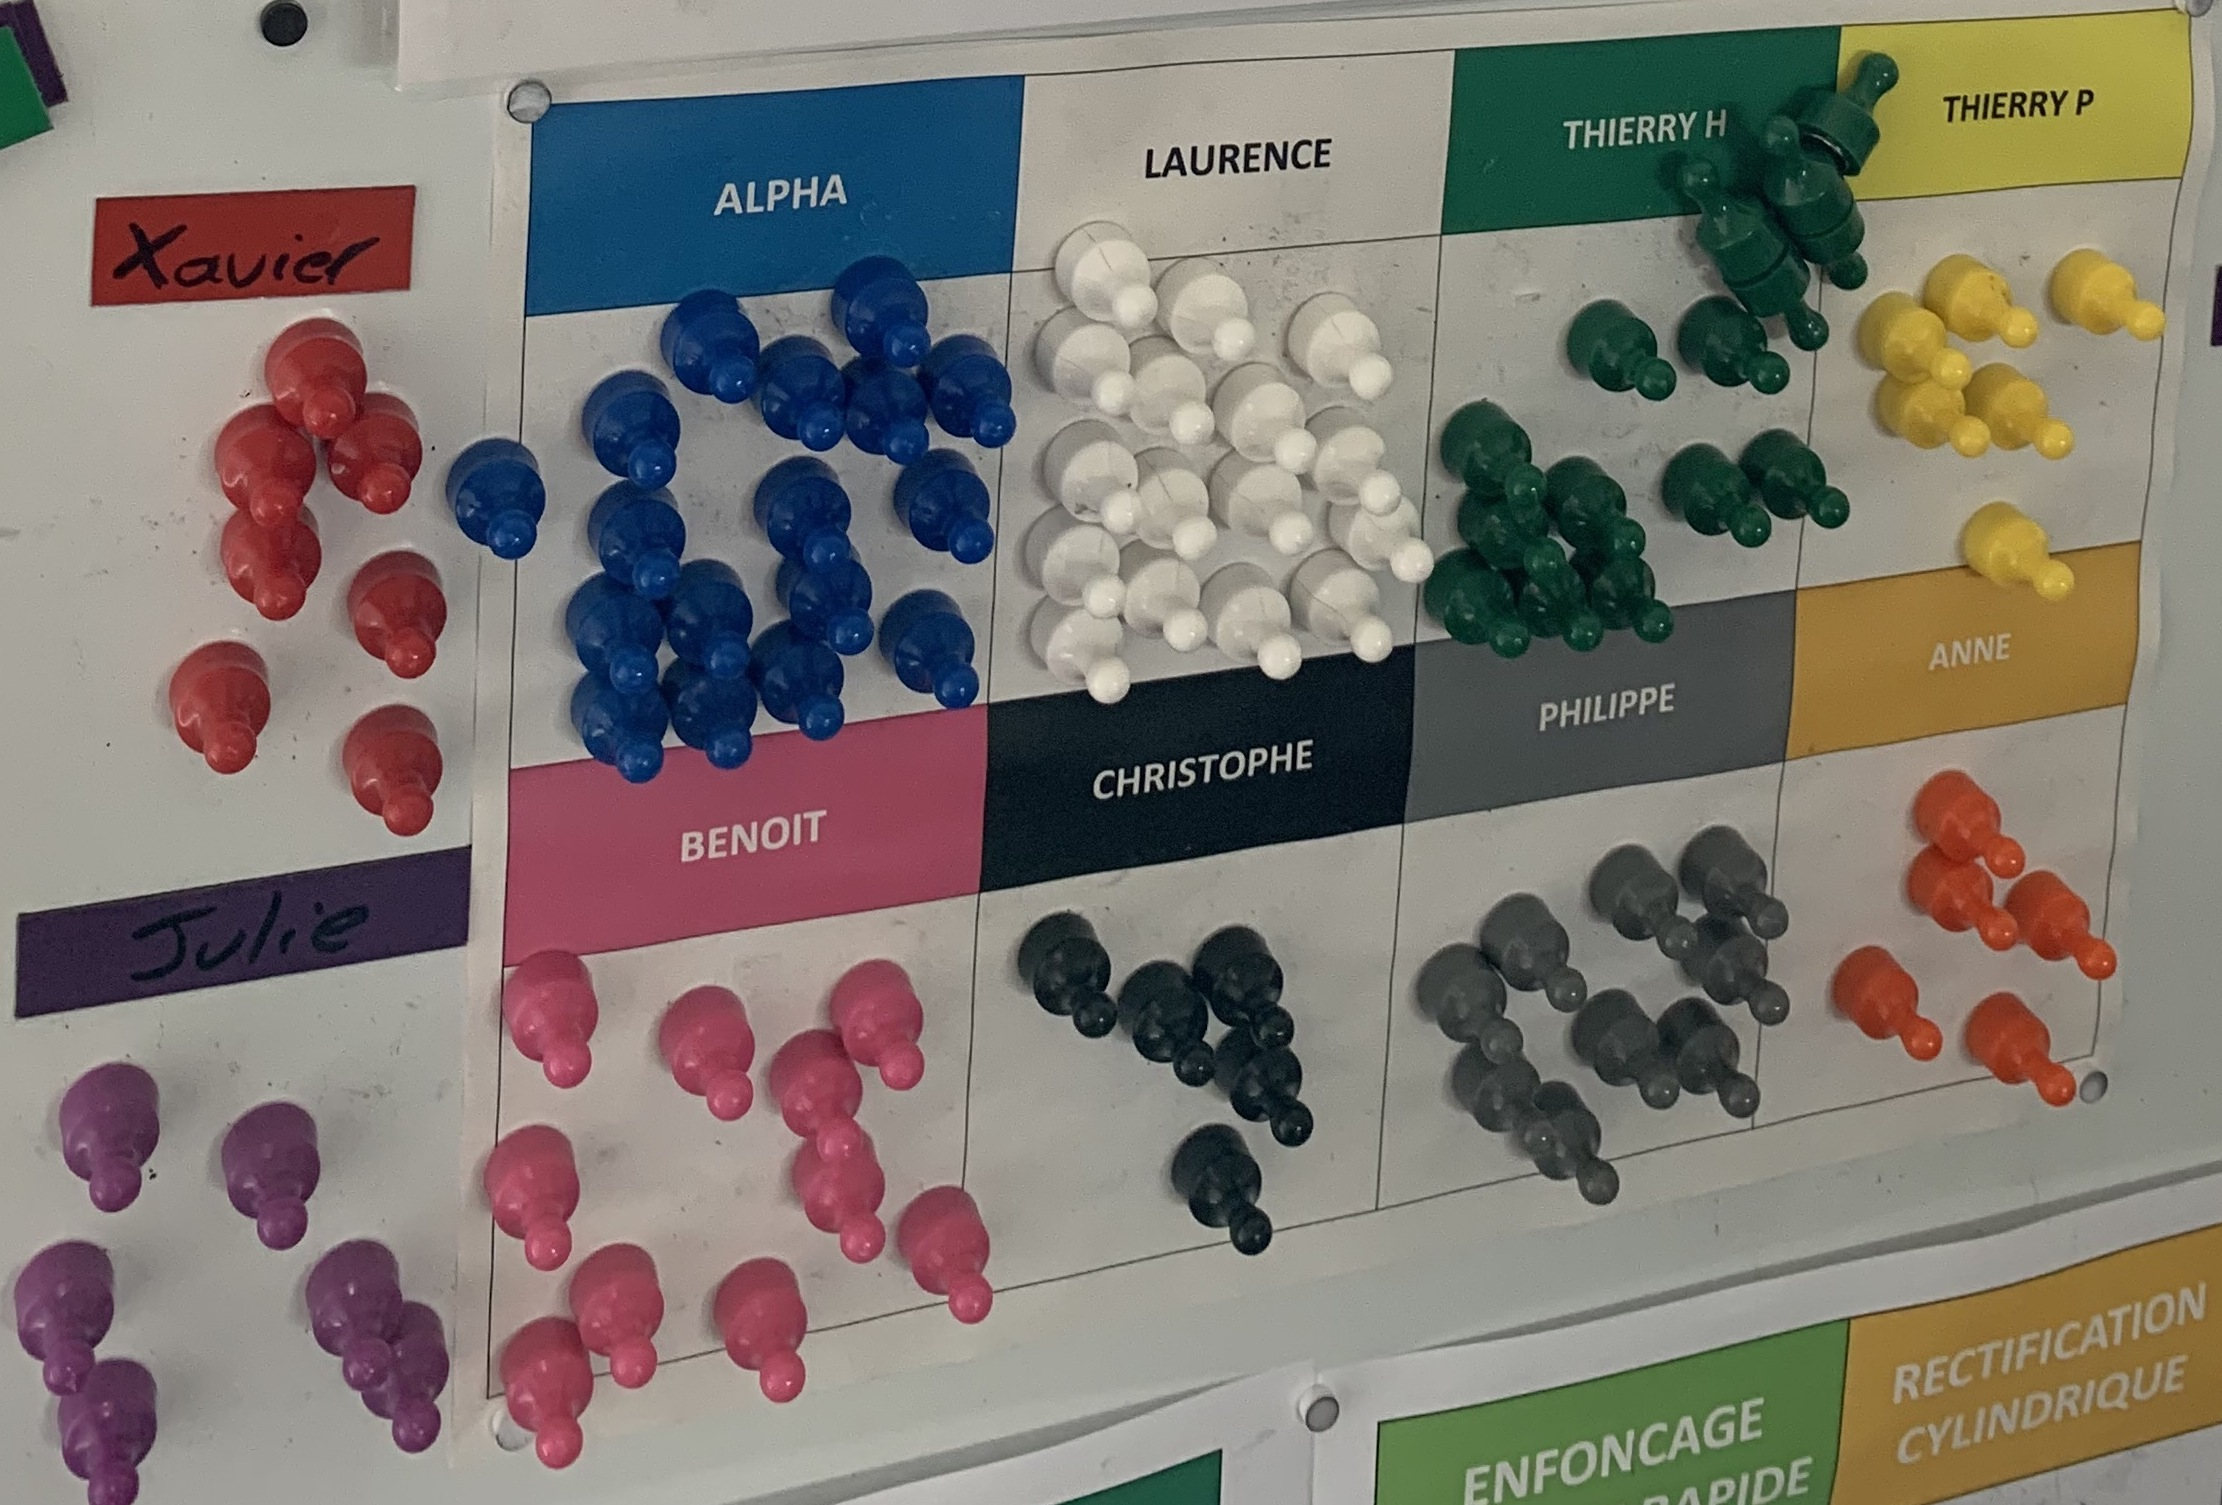
\includegraphics[scale=0.15]{img/employee.jpg}
    \caption{Chaque employé a sa couleur d'épingle pour identifier ses missions}
    \label{fig:employee}
\end{figure}

\hfill \\
Cet outil a permis à Panorama de se démarquer de ses concurrents (comme "maboutiqueenlean"\cite{MaBoutiqueEnLean} par exemple) qui eux, ne font pas réellement de l'accompagnement global des TPE personnalisé.


\clearpage
\subsubsection*{Problématique}
Mais la version actuelle du séquenceur soulève plusieurs problèmes : 
\begin{itemize}
    \item Il est encombrant
    \item L'aspect “papier/crayon" repousse les entreprises
    \item Son utilisation est gourmande en temps
\end{itemize}

C'est pourquoi Panorama Performance s'est posé la question d'un possible passage à une solution informatique reprenant les éléments clés de cet outil. L'application qu'ils souhaiteraient mettre place devra permettre de laisser les collaborateurs réfléchir aux modifications qui les arrangent et interagir entre eux pour trouver leur propre façon de gérer la production de manière optimisée. Panorama Performance a fortement insisté sur le fait qu'il nous fallait \textbf{digitaliser et conserver les fonctionnalités actuelles sans automatiser} !\\

La dernière proposition de valeur de ce projet serait de pouvoir mettre en place, un backup des données des utilisateurs (délais de livraison, disponibilité des machines, productivité, \dots) Cela permettra, grâce à ces informations, à la demande des clients, de créer des indicateurs qui permettront, d'améliorer encore la performance.

